%%%%%%%%%%%%%%%%%%%%%%%%%%%%%%%%%%%%%%%%%
% Large Colored Title Article
% LaTeX Template
% Version 1.1 (25/11/12)
%
% This template has been downloaded from:
% http://www.LaTeXTemplates.com
%
% Original author:
% Frits Wenneker (http://www.howtotex.com)
%
% License:
% CC BY-NC-SA 3.0 (http://creativecommons.org/licenses/by-nc-sa/3.0/)
%
%%%%%%%%%%%%%%%%%%%%%%%%%%%%%%%%%%%%%%%%%

%----------------------------------------------------------------------------------------
%	PACKAGES AND OTHER DOCUMENT CONFIGURATIONS
%----------------------------------------------------------------------------------------

\documentclass[DIV=calc, paper=a4, fontsize=11pt, twocolumn]{scrartcl}	 % A4 paper and 11pt font size

\usepackage{lipsum} % Used for inserting dummy 'Lorem ipsum' text into the template
\usepackage[english]{babel} % English language/hyphenation
\usepackage[protrusion=true,expansion=true]{microtype} % Better typography
\usepackage{amsmath,amsfonts,amsthm} % Math packages
\usepackage[svgnames]{xcolor} % Enabling colors by their 'svgnames'
\usepackage[hang, small,labelfont=bf,up,textfont=it,up]{caption} % Custom captions under/above floats in tables or figures
\usepackage{booktabs} % Horizontal rules in tables
\usepackage{fix-cm}	 % Custom font sizes - used for the initial letter in the document

\usepackage{sectsty} % Enables custom section titles
\allsectionsfont{\usefont{OT1}{phv}{b}{n}} % Change the font of all section commands

\usepackage{fancyhdr} % Needed to define custom headers/footers
\pagestyle{fancy} % Enables the custom headers/footers
\usepackage{lastpage} % Used to determine the number of pages in the document (for "Page X of Total")
\usepackage{paralist}
\usepackage{graphicx}
% Headers - all currently empty
\lhead{}
\chead{}
\rhead{}

% Footers
\lfoot{}
\cfoot{}
\rfoot{\footnotesize Page \thepage\ of \pageref{LastPage}} % "Page 1 of 2"

\renewcommand{\headrulewidth}{0.0pt} % No header rule
\renewcommand{\footrulewidth}{0.4pt} % Thin footer rule

\usepackage{lettrine} % Package to accentuate the first letter of the text
\newcommand{\initial}[1]{ % Defines the command and style for the first letter
\lettrine[lines=3,lhang=0.3,nindent=0em]{
\color{DarkGoldenrod}
{\textsf{#1}}}{}}

%----------------------------------------------------------------------------------------
%	TITLE SECTION
%----------------------------------------------------------------------------------------

\usepackage{titling} % Allows custom title configuration

\newcommand{\HorRule}{\color{DarkGoldenrod} \rule{\linewidth}{1pt}} % Defines the gold horizontal rule around the title

\pretitle{\vspace{-30pt} \begin{flushleft} \HorRule \fontsize{50}{50} \usefont{OT1}{phv}{b}{n} \color{DarkRed} \selectfont} % Horizontal rule before the title

\title{Fiducial Markers} % Your article title

\posttitle{\par\end{flushleft}\vskip 0.5em} % Whitespace under the title

\preauthor{\begin{flushleft}\large \lineskip 0.5em \usefont{OT1}{phv}{b}{sl} \color{DarkRed}} % Author font configuration

\author{Bruno Maia, Jo\~{a}o Costa, } % Your name

\postauthor{\footnotesize \usefont{OT1}{phv}{m}{sl} \color{Black} % Configuration for the institution name
Faculty of Engineering of the University of Porto % Your institution

\par\end{flushleft}\HorRule} % Horizontal rule after the title

\date{} % Add a date here if you would like one to appear underneath the title block

%----------------------------------------------------------------------------------------

\begin{document}

\maketitle % Print the title

\thispagestyle{fancy} % Enabling the custom headers/footers for the first page 

%----------------------------------------------------------------------------------------
%	ABSTRACT
%----------------------------------------------------------------------------------------

% The first character should be within \initial{}
\initial{F}\textbf{iducial markers are usually divided in two distinct application: either to store information (such as QRCodes) or for perspective calculations (such as the ARToolkit markers).
In this work we present an hybrid marker, that allows for both information storage and Augmented Reality applications.}

%----------------------------------------------------------------------------------------
%	ARTICLE CONTENTS
%----------------------------------------------------------------------------------------

\section*{Introduction}

In a practical approach the two most common technologies used by Augmented reality (AR) for pinpoint where to deploy digital content in real-time video frames are georeferentiation and Computer Vision (CV) techniques. Although  applied in some marketing and entertainment mobile applications,  the use of CV techniques in real-world situations is
difficult due to several constraints like scenario mutation over time, high visual noise or lack of unchanged anchor points.
 

Despite these difficulties, AR supported on CV is growing with the development of new frameworks and powerful new algorithms. This evolution, combined with sophisticated mobile devices, leads us to believe It's time to take Computer Vision and Augmented Reality to different industries , using its potential to solve a wider array of problems.


%------------------------------------------------

\section*{Goals}

This project’s goals can be summarized by the:
\begin{itemize}
\item Detecting of a singular fiducial marker.
\item Tracking of a singular fiducial marker.
\item Augmenting the fiducial marker with an image.
\item Displaying the identifier encoded in the fiducial marker.
\end{itemize}

There are a few restrictions to be taken into consideration such as:
\begin{itemize}
\item The detection/tracking must be done with a mobile smartphone which presents reduced processing power.
\item The fiducial marker size must be small.
\item The fiducial marker should be recognized from at least 1 meter away.
\item The detection/tracking must be implemented by using OpenCV4Android.
\item The algorithm should perform in real time, i.e. framerate must be sustainable and should be optimized.
\end{itemize}
%------------------------------------------------

\section*{Solution}

The solution is divided into 2 parts:


\begin{inparaenum}[(i)]
\item The Encoder part, which handles the conversion of an unique id (in our implementation, simply a number between 0 and $2^{15} - 1$) into a unique fiducial marker with redundancy. 


\item The Decoder part, which is an android application which scans and detects fiducial markers and augments them with an image while displaying the stored unique identifier.
\end{inparaenum}

%------------------------------------------------

\subsection*{Fiducial Marker}
The fiducial marker opted for is a matrix-like representation where its tracking points are achieved by the means of four colored cells in the corners of the matrix (3 green and 1 red) as seen in figure~\ref{fig:marker1}.

\begin{figure}[!h]
    \centering
    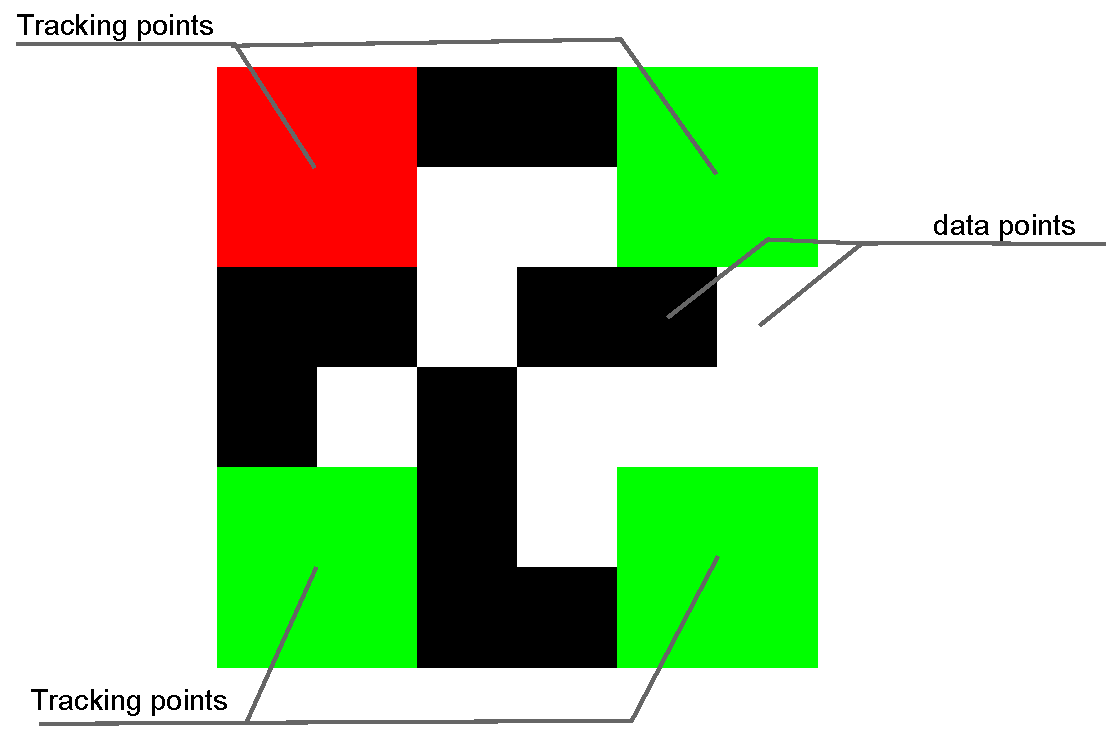
\includegraphics[width=0.9\columnwidth]{marker1.pdf}
    \caption{Fiducial marker's types of cells}
    \label{fig:marker1}
\end{figure}

The selected colors for the tracking points provide for optimal contrast and are bigger than data points to facilitate tracking. 


It's composed by an 6x6 cell matrix which gives us 20 cells when we take the tracking cells. From these 20 cells, which we can equate to one bit each, we’ve spliitted 15 bits for the identificator ($2^{15} = 32768$ possibilities) and 5 bits for redundancy as seen in figure~\ref{fig:marker2}.

\begin{figure}[!h]
    \centering
    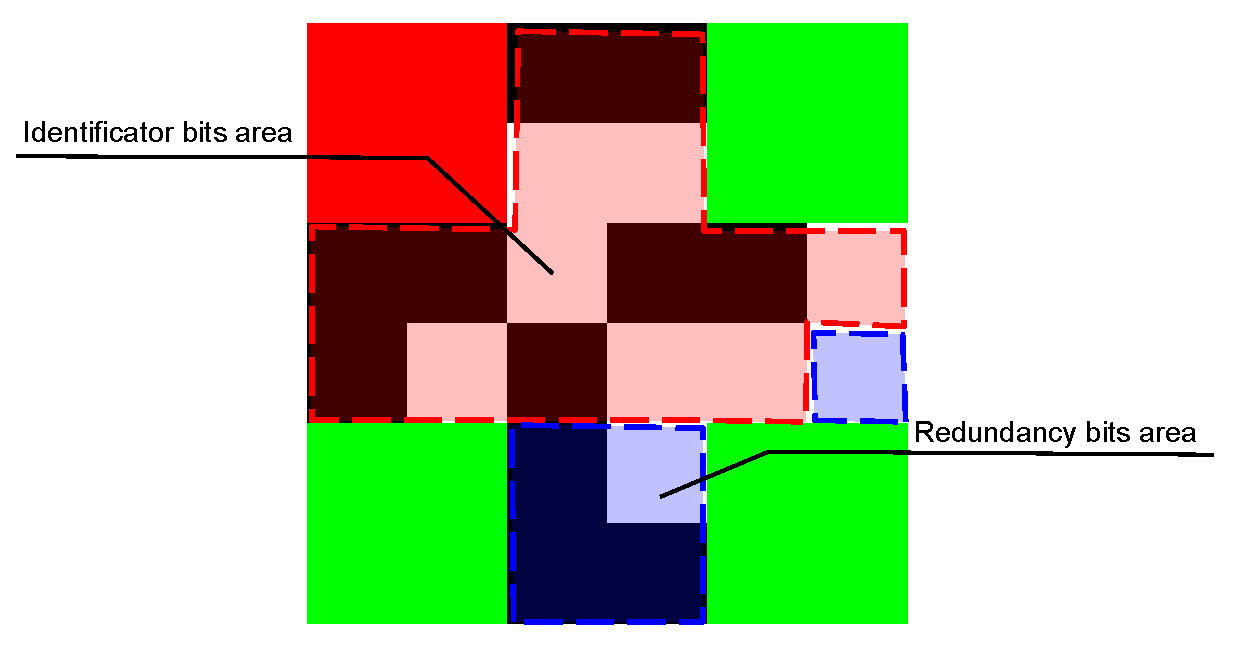
\includegraphics[width=1.0\columnwidth]{marker2.pdf}
    \caption{Fiducial marker's areas of data}
    \label{fig:marker2}
\end{figure}

The representation is read from left to right, and from top to bottom and is set in a way that the less significant bit is the first one as seen in figure~\ref{fig:bits}.

\begin{figure}[!h]
    \centering
    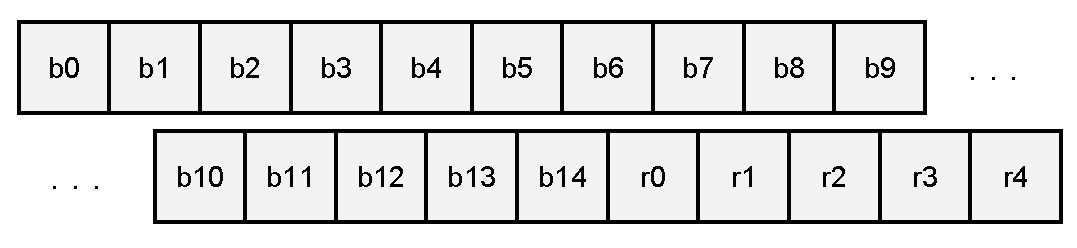
\includegraphics[width=0.9\columnwidth]{bits.pdf}
    \caption{Data representation format}
    \label{fig:bits}
\end{figure}

The 5 bits used for redundancy allow us to code our message using a Hamming(31,26) code, and therefore we are able to either correct 1-bit errors or detect 2-bit errors.

\subsection*{Marker Encoder}

The encoder program was made in C++ and its usage is as such:
\begin{verbatim}
decoder <identifier> [output_file_name]
\end{verbatim}


We pass it an unique number which will be stored within the fiducial mark and we can also specify the output filename, otherwise it will default to ``default.bmp''. The successful output artifact of the program is an bmp containing the fiducial mark encoded with the identifier.

\subsection*{Marker Decoder}
The decoder was written in Java with OpenCV.

The decoder works in two phases: A detection phase and a tracking phase.\\


The detection phase is the most intensive, and therefore the decoder starts by downsampling the image by a factor of 4. It then converts it to HSV and extracts the red and green blobs via a simple inRange filter and a closing operation.\\


After that, the red and green blobs are extracted using a flood fill algorithm, and their centroids are roughly estimated based on their top-left corner and their area (Note: using a different blob detection algorithm, it might be possible to extract the correct centroids and have a faster running time, although there's no fast blob detector in OpenCV).\\


Next, we calculate the correct points in the following way:
for each red blob r in R
for each green blob g in G
create a line l between r and g, with center c
trace a line n perpendicular to l that goes through c
create two point estimates, g’1 and g’2, which are the points of n with d(c,g’1) = d(c,g’2) = d(r,c), with g1!=g’2
pick the two points, g1,g2 in G which are closest to g’1 and g’2 (respectively).
if d(g1,g’1) and d(g2,g’2) are small enough, then a marker was found with colored corners centered in [r,g1,g,g2].\\

\begin{figure}[!h]
    \centering
    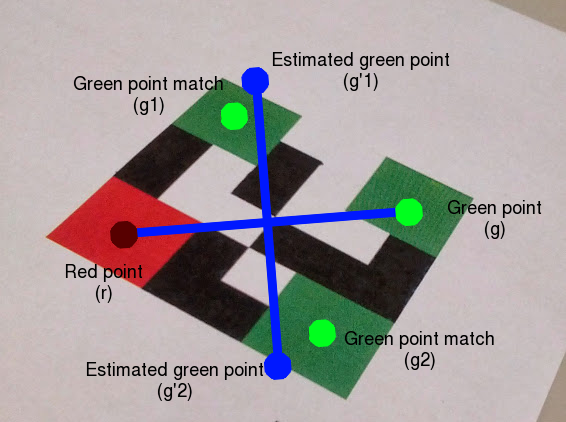
\includegraphics[width=0.9\columnwidth]{marker.png}
    \caption{Data representation format}
    \label{fig:marker3}
\end{figure}

We continue with the homography between the marker and the image is calculated (taking into account that the detected points are the corner centers and not the marker's corners).
Once the detection is successful, the detector goes into the tracking phase.\\


The tracking phase takes into account the previously detected points to update the marker position. To do this, it fetches 4 small regions from the image, one for each of the previously detected points (the size of these regions depend on the size of the detected marker).\\


It's assumed that each region will only contain one blob, and therefore all the values that pass the inRange test are used to calculate the region centroid (this time correctly calculated).\\


This new centroids are interpolated with the previously detected coordinates using a constant weight, so that there's a smooth transition between frames. The homography is recalculated using this new points.\\


After each homography calculation, the inverse of the homography is used to read the marker's content.\\


\section*{Tests}

A series of tests were made throughout and after the completion of the project. Among these, a set of approaches were found that weren't considered as performant as the final, proposed one.

The tests were performed with a Galaxy Nexus ( Dual-core 1Ghz, 1Gb RAM) which is less powerful than the probable hardware that the program will run as specified in the problem description ( Quad-core and 1Gb RAM ).

\subsection*{Less performant approaches}
Here, we'll explore some of the approaches we took and ultimately left and its reasons:

\begin{description}
\item[Smaller tracker cells]
Initially, the tracking cells were only 1 cell wide and the matrix size was only 5x5 which gave us a 25 which gave us a 25-4 = 21 bits for the identifier and the redundancy.
We're having problems tracking the marker at longer distances and final solution provided better results with only 1 bit lost for the identifier.

\item[Ndk performance]
At first, we developed our algorithm in C++ using the laptop camera and later ported it for android. This resulted in poor performance. Migrating the code for the Java API which performed better and simplified the code and building process.

\item[Parallel multithreaded processing]
When trying to optimize the framerate and the algorithm, we've explored the possibility of parallel multi threading. This, theoretically, would enable us optimize the camera framerate by sending each camera frame caught to a thread pool of the size of the number of processors on the device as seen in figure~\ref{fig:threading} mitigating the framerate slowdown by a delay in the output image. 

\begin{figure}[!h]
    \centering
    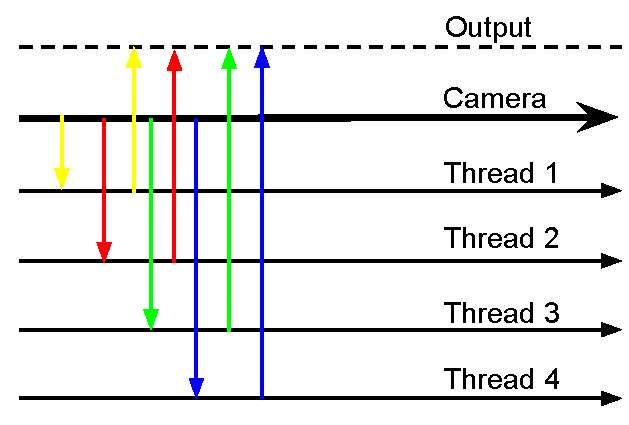
\includegraphics[width=0.9\columnwidth]{threading.pdf}
    \caption{Diagram of camera augmenting interpolation}
    \label{fig:threading}
\end{figure}

We've extended a thread to have all the required memory allocations for our openCV matrices, so they wouldn't have to be re-allocated at each iteration and try to boost our application.
Ultimately, while testing this showed a poorer performance.

\end{description}

\subsection*{Detection results}
Here, we show the augmenting of the image caught by the smartphone camera with the PT logo and the number encoded in the fiducial marker.

\begin{figure}[!h]
    \centering
    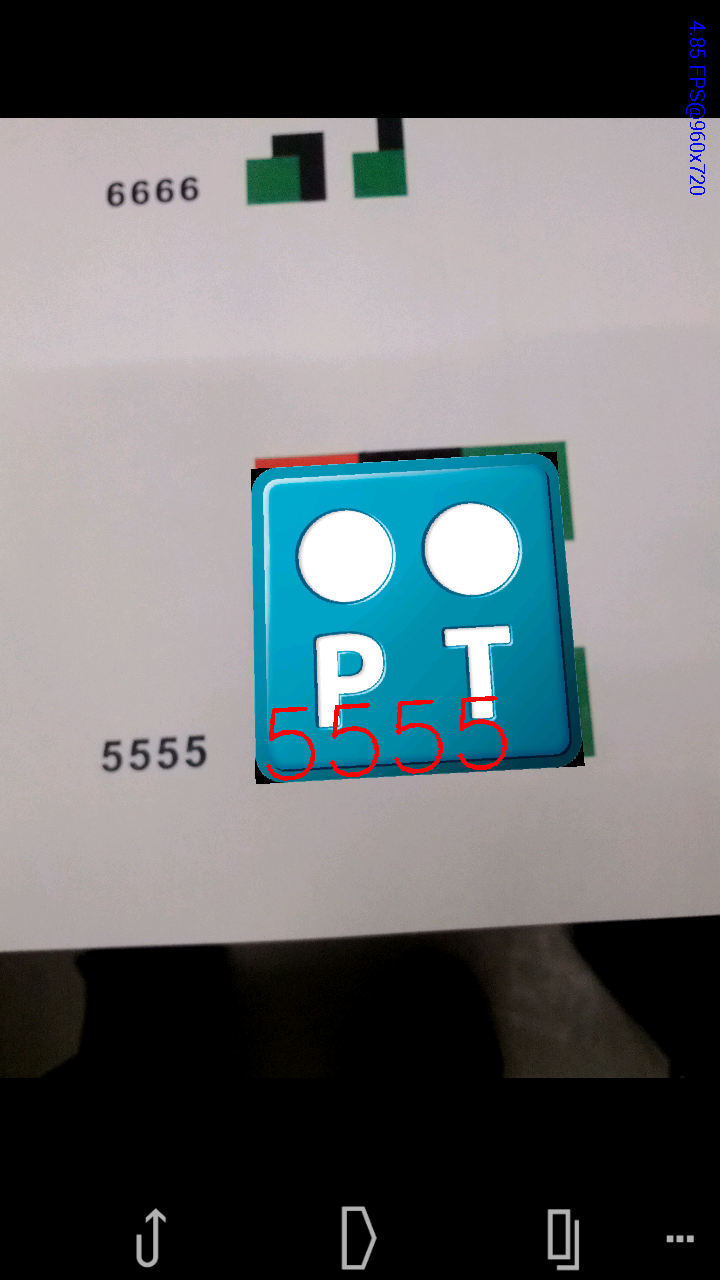
\includegraphics[width=0.6\columnwidth]{phone.png}
    \caption{Smartphone screenshot of image detection and it's augmentation}
    \label{fig:phone}
\end{figure}

\section*{Conclusion}
We think this implementation clears all goals and requirements of the project. Even though we optimized the program, we wished we could had improved even further the framerate. Perhaps our multithreaded approach would be a good point to further explore and with the correct tweaking may had yielded better results.

Any question related to any of the work may and should be forwarded to the contact email.


\end{document}